\section{Experimental Results}
\label{sec:experiments}
In this section, we evaluate the posterior approximation quality achieved by
pseudocoreset sparse VI (\psvi) compared against uniform random subsampling~(\uniform), Hilbert
coresets~(\giga~\citep{campbell18}) and \sparsevi~greedy coreset
construction~\citep{campbell19neurips}.  For black-box constructions of \sparsevi~and \psvi~we used $S =
100$ Monte Carlo samples per gradient estimation. For \giga~we used a
100-dimensional random projection from a Gaussian approximate posterior $\hpi$
with  two choices for mean and covariance: one set to the exact
posterior~(\optimal), which is not tractable to obtain in practice and forms an
optimistic estimate of achievable approximation quality; and one with mean and
covariance set to a random point on the interpolant between the prior and the
exact posterior point estimates, and subsequently corrupted with $75\%$
additive relative noise~(\realistic). Notably, Hilbert coresets and
\sparsevi~develop incremental schemes for construction, while \psvi~relies on
batch optimization with random initialization~(\cref{alg:psvi}), and does not
use any information from pseudocoresets of smaller size. An incremental scheme
for \sparsevi~is included in~\cref{app:experiments_appendix}. %Code for the presented experiments is available at~\href{https://github.com/dionman/psvi}{https://github.com/dionman/psvi}. 

\subsection{Gaussian mean inference}
\label{section:gaussian_experiment}

We first evaluate the performance of \psvi~on a synthetic dataset of ${N =10^3}$ datapoints, where we aim
to infer the posterior mean $\theta \sim \distNorm(\mu_0, \Sigma_0)$ of a \mbox{$ d$-dimensional} Gaussian conditioned
on Gaussian observations $(X_n)_{n=1}^N \distiid \distNorm(\theta, \Sigma)$. 
 In this example, the exact pseudocoreset posterior for any set of weights
$(w_m)_{m=1}^M$ and pseudopoint locations $(u_m)_{m=1}^M$ is available in
closed-form:
\[
\Sigma_{u,w} &= ( \Sigma_0^{-1} + \sum_{m=1}^{M}  w_m \Sigma^{-1}
)^{-1} & \mu_{u,w} &= \Sigma_{u,w} (\Sigma_{0}^{-1} \mu_0 + \Sigma^{-1}
\sum_{m=1}^{M} w_m u_m).
\]
 Using the exact posterior, we derive the exact
moments used in the gradient formulae from \cref{eq:dkl_duw} in closed form
(see~\cref{app:gaussian_experiment_appendix}),
\[ 
\begin{aligned}
& \cov_{u,w}[f_n ,f_m]  =  v_n^T \Psi v_m + \half \tr{\Psi^T \Psi},
& \cov_{u,w}[\tf_n ,f_m]  =  \tv_n^T \Psi v_m + \half \tr{\Psi^T \Psi},\\
& \cov_{u,w}[h(u_i), f_n] = Q^{-T}\Psi v_n,
& \cov_{u,w}[h(u_i), \tf_n] = Q^{-T}\Psi \tv_n,
\end{aligned}\label{eq:synthgaussformulae}
\]
where $Q$ is the Cholesky decomposition of $\Sigma$ (i.e.~$\Sigma = QQ^T$),
$\Psi \defined Q^{-1}\Sigma_{u,w} Q^{-T}$,
$v_n := Q^{-1}(x_n - \mu_{u,w})$, and 
$\tv_m := Q^{-1}(u_m - \mu_{u,w})$. 
%
\begin{figure*}[!t]
	\centering
	\begin{subfigure}[c]{.29\textwidth}
			\centerline{\scalebox{1}{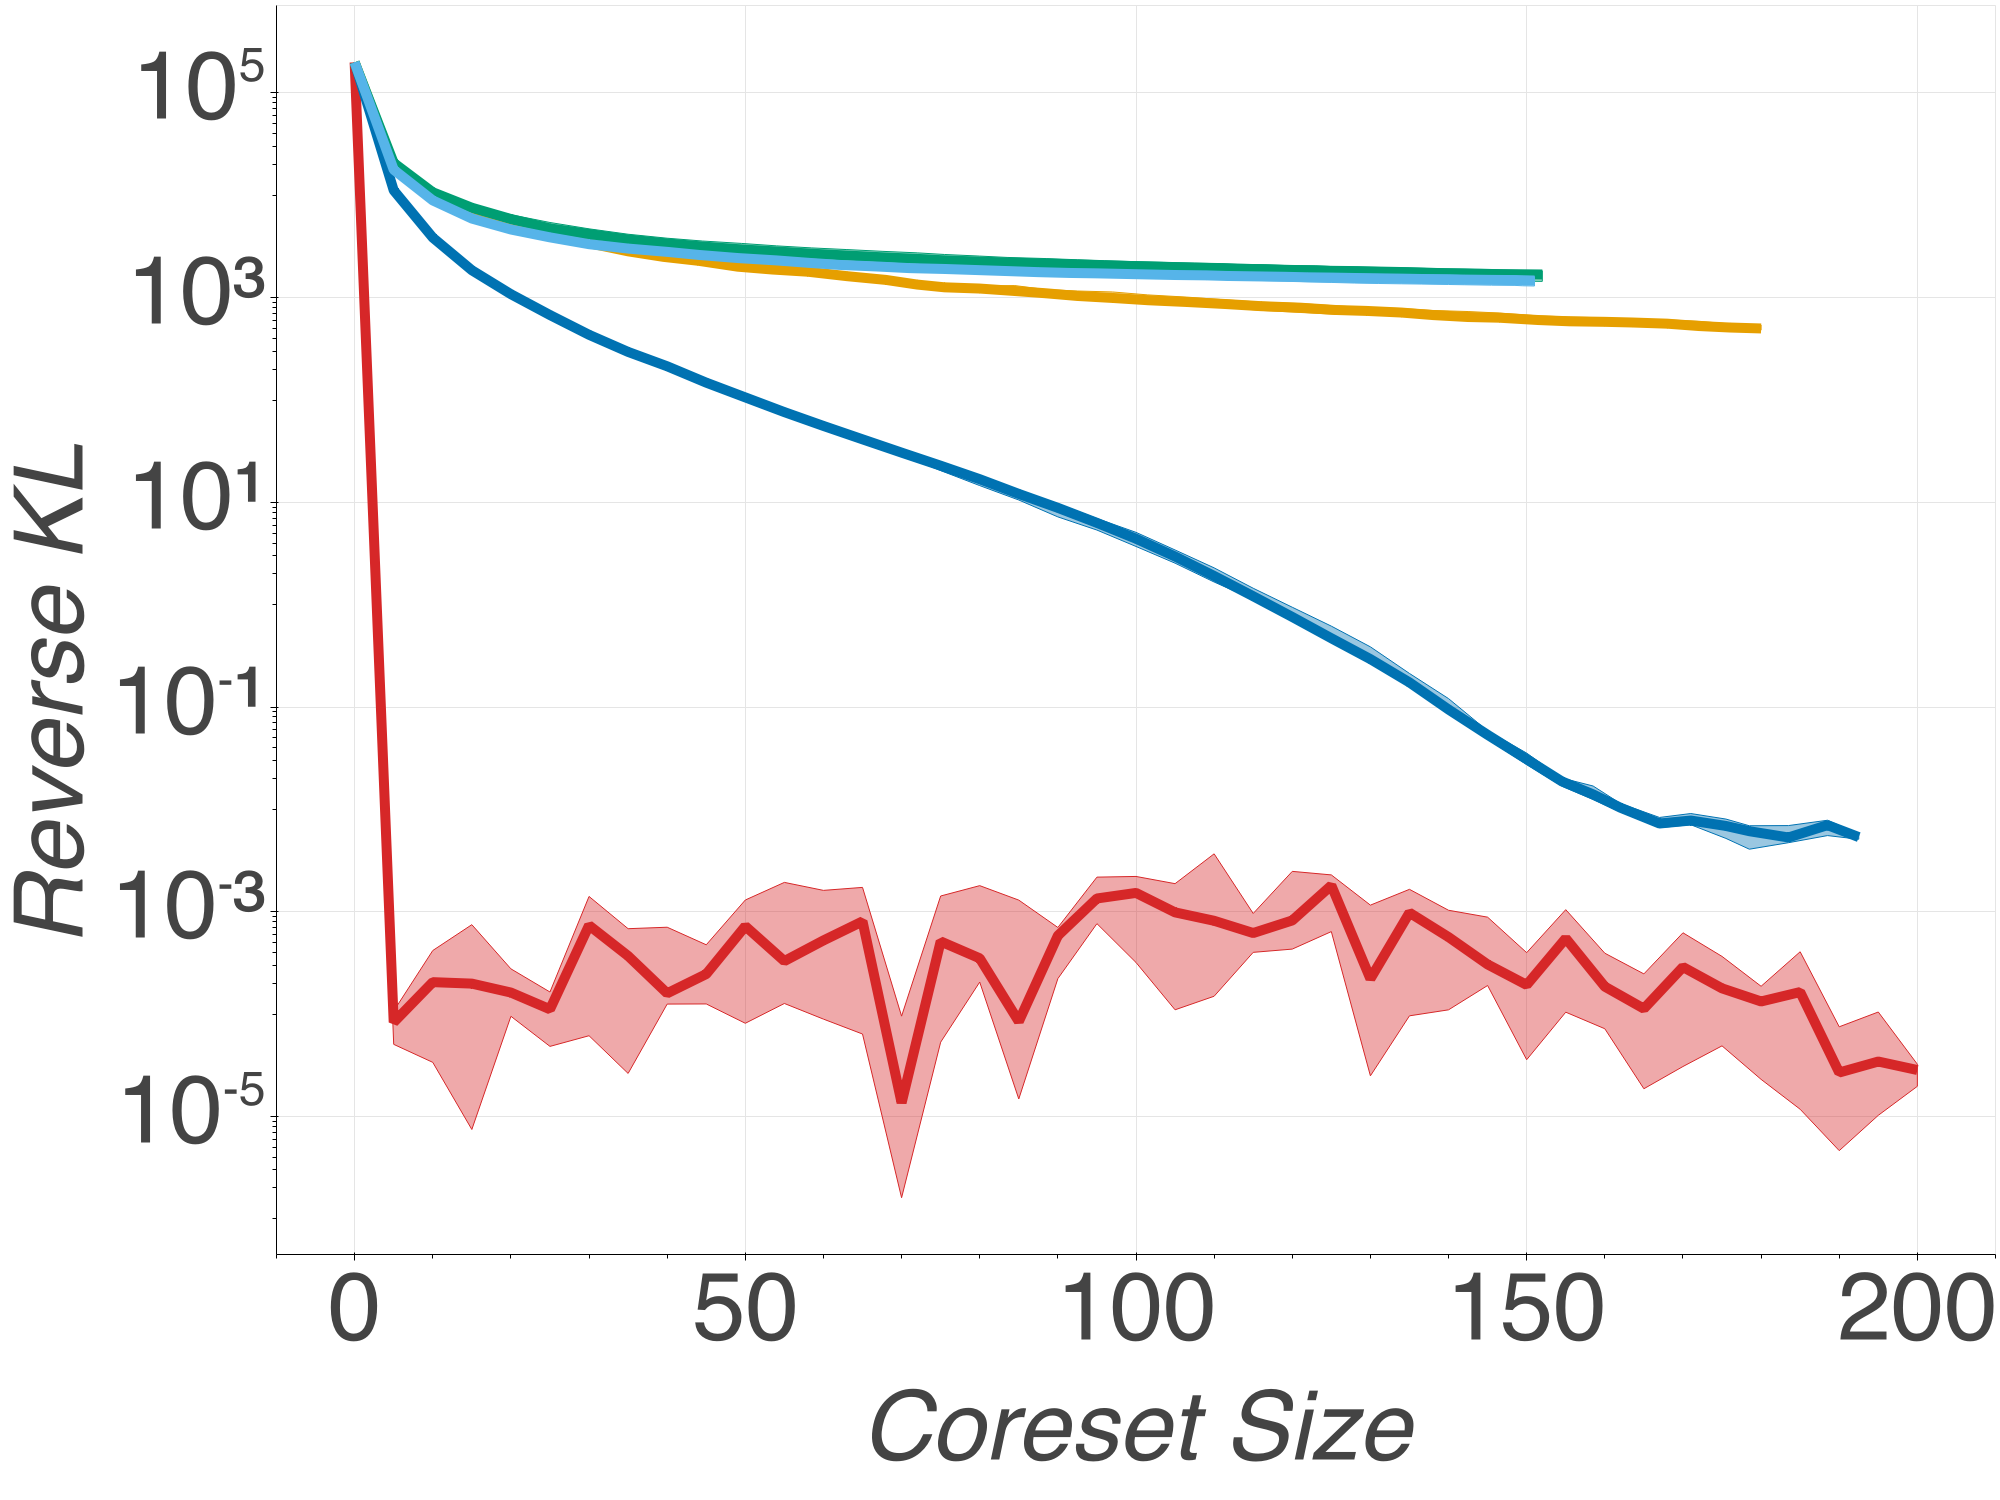
\includegraphics[ width=1.15\columnwidth]{\MyPath/figs/d200_KLDvsCstSize.png}}}%
                       \caption{(a) Gaussian mean inference, $d=200$\label{fig:gauss_mean_200}}
	\end{subfigure}\hfill\qquad
	\begin{subfigure}[c]{.29\textwidth}
			\centerline{\scalebox{1}{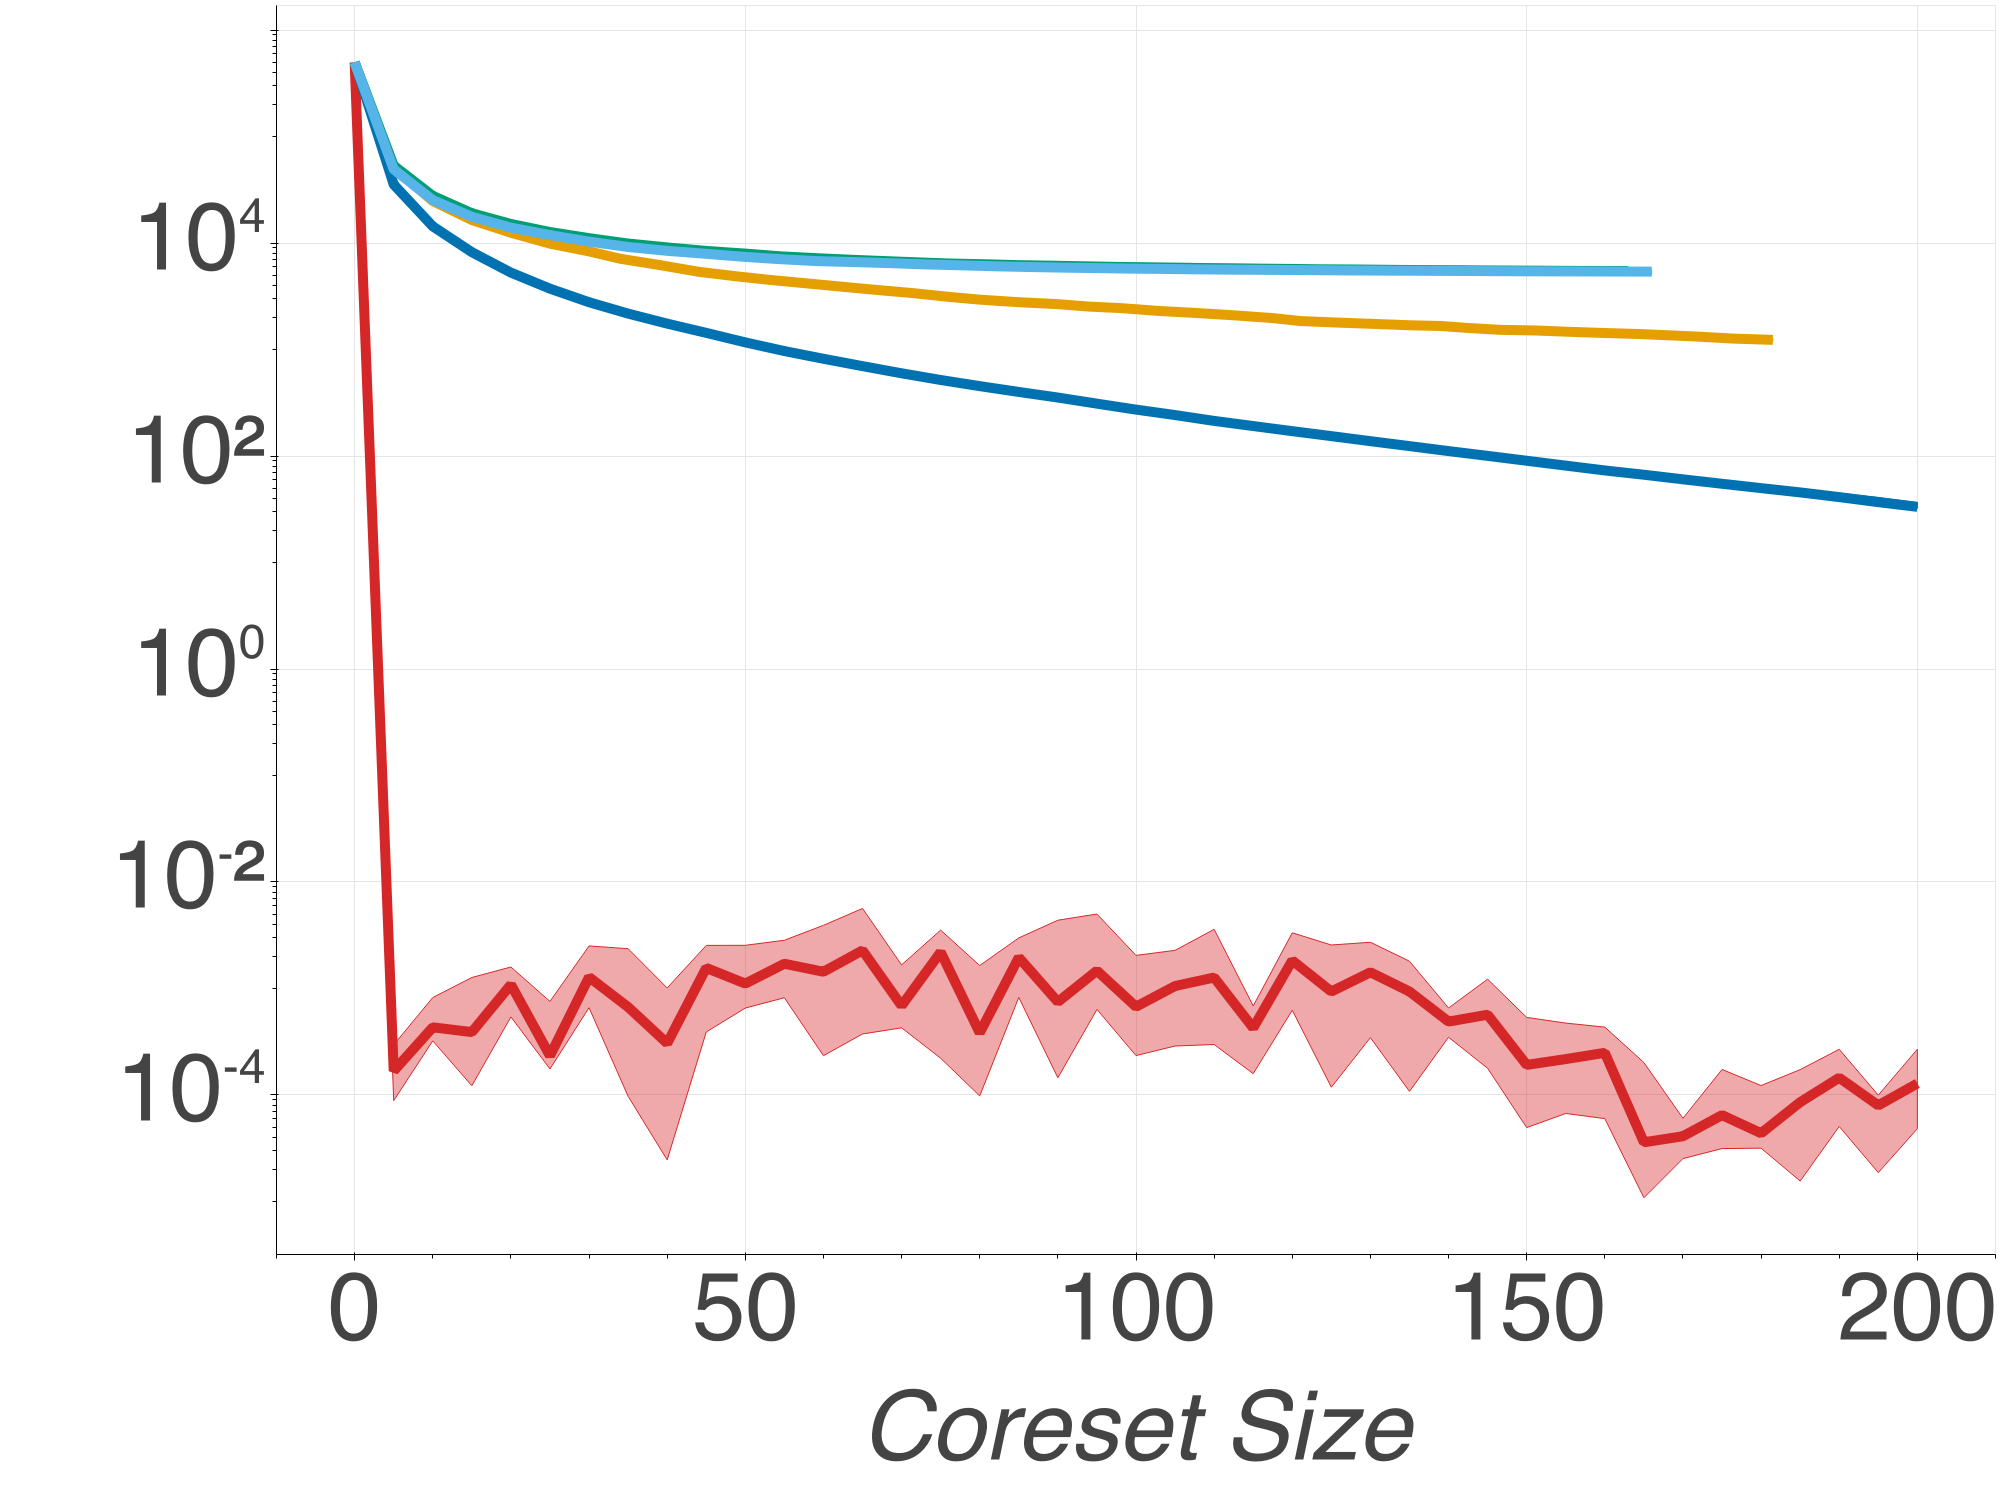
\includegraphics[ width=1.15\columnwidth]{\MyPath/figs/d500_KLDvsCstSize.png}}}%
				\caption{(b) Gaussian mean inference, $d=500$\label{fig:gauss_mean_500}}
	\end{subfigure}\hfill\qquad
	\begin{subfigure}[c]{.29\textwidth}
			\centerline{\scalebox{1}{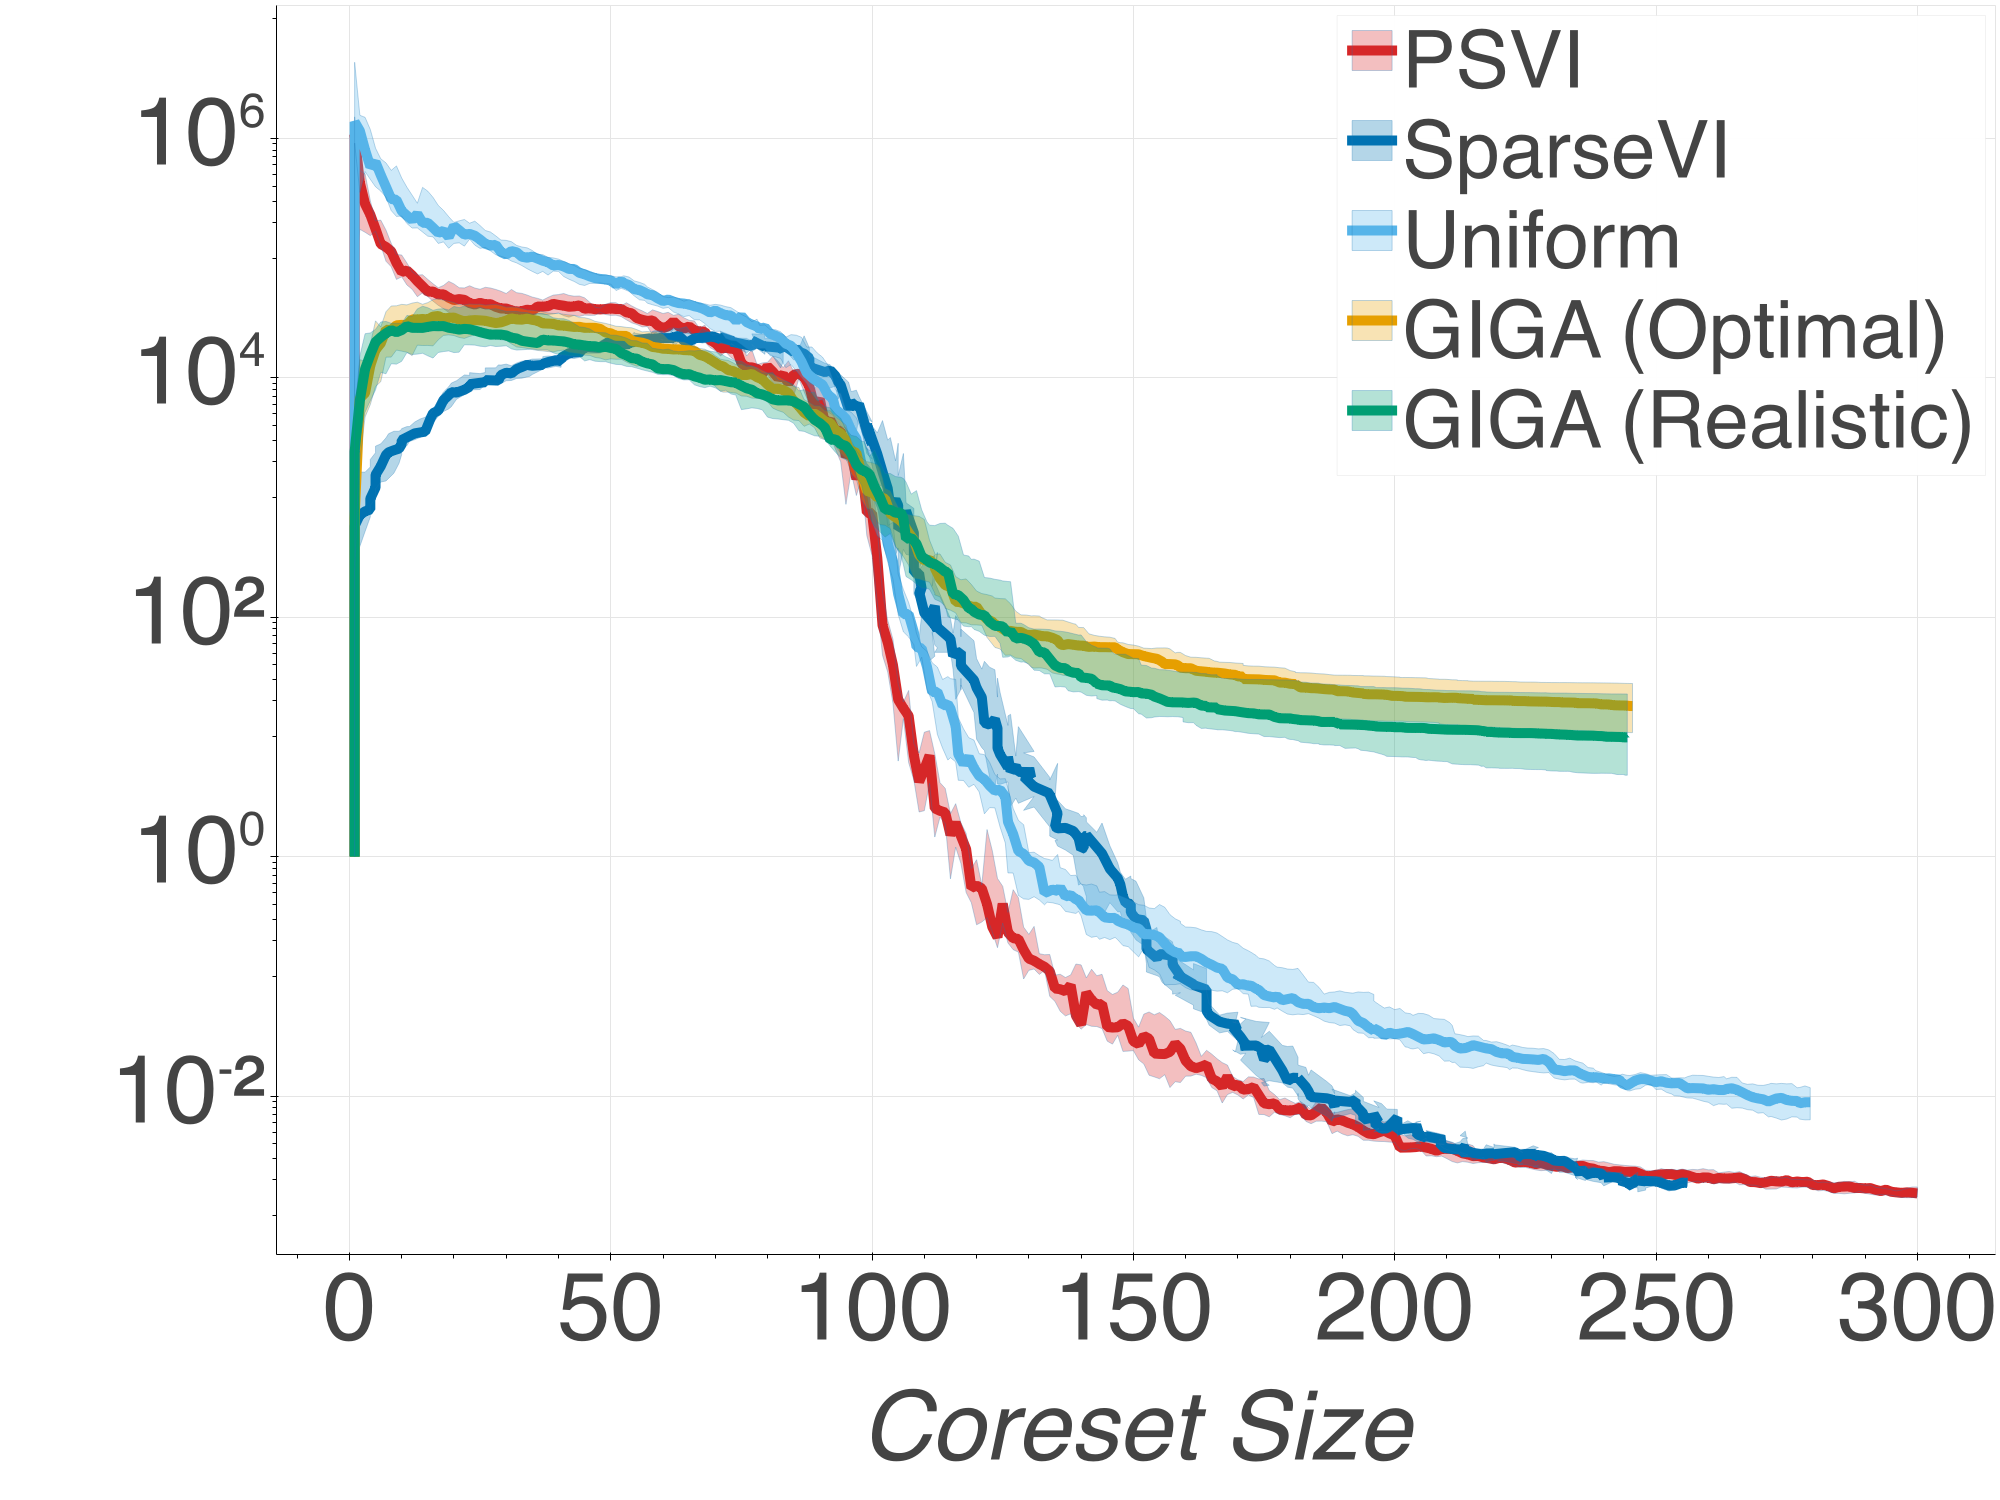
\includegraphics[width=1.15\columnwidth]{\MyPath/figs/linregTT_KLDvssz.png}}}%
				\caption{(c) Bayesian linear regression, $d=100$\label{fig:linreg_300}}
  \end{subfigure}
	\caption{Comparison of coreset approximate posterior quality for experiments on synthetic datasets over {10 trials}. Solid lines display the median KL divergence, with shaded areas showing~$25^{\text{th}}$ and~$75^{\text{th}}$ percentiles of KL divergence. In \cref{fig:linreg_300}, KL divergence is normalized by the prior.}
	\label{fig:gaussian_dkl}
\end{figure*}
%
We vary the pseudocoreset size from $M=1$ to $200$, and set the total number of
iterations to $ T =  500$. We use learning rates $ \gamma_t(M) = \alpha(M)
t^{-1}$, where  $ \alpha(M) = 1 $ for \sparsevi~and $ \alpha(M) = \max(1.1 - 0.005M, 0.2)
$ for \psvi.  As verified in~\cref{fig:gauss_mean_200,fig:gauss_mean_500},
Hilbert coresets provide poor quality summarizations in the high-dimensional
regime, even for large coreset sizes.  Despite showing faster decrease of
approximation error for a larger range of coreset sizes, \sparsevi~is also
fundamentally limited by the use of the original datapoints, per
\cref{prop:original_coreset_fails}.  Furthermore, we observe that the quality of all
previous coreset methods when $d=500$ is significantly lower
compared to $d=200$. On the other hand, the KL divergence for  \psvi~decreases
significantly more quickly, giving a near perfect approximation for true
posterior with a single pseudodata point regardless of data dimension. As
shown earlier in~\cref{fig:gaussian_coreset_points}, \psvi~has the capacity to move the
pseudodata points in order to capture the
true posterior very efficiently. 

\subsection{Bayesian linear regression}
\label{section:linreg_experiment}
In the second experiment, we use a set of ${N=2,000}$ 
$101$-dimensional datapoints $(x_n,y_n)_{n=1}^{N}$ generated as follows: $(x_n)_{n=1}^N  \distiid \distNorm(0, I),\; (y_n)_{n=1}^N  \dist [1, x_n]^T\theta + \epsilon_n,\;  (\epsilon_n)_{n=1}^{N} \distiid \distNorm(0, \sigma^2)$, and aim to infer $\theta \in \reals^{101}$. We assume a prior $\theta \dist \distNorm(\mu_0,\sigma_0^2 I)$, where $ \mu_0, \sigma_0^2$ are the dataset empirical mean and second moment, and set the noise parameter $ \sigma$ to the variance of $(y_n)_{n=1}^{N}$. We apply stochastic optimization for \psvi~construction~(also see~\cref{app:linreg_model_appendix}). We use learning rates $\gamma_t = t^{-1}$ for \sparsevi, and $\gamma_t = 0.1t^{-1}$ for \psvi, $B=200$, $T=1000$, while selection step for \sparsevi~is carried out over the full dataset. \cref{fig:linreg_300} shows that Hilbert coresets cannot improve posterior approximation in this setting with 100 random projections (see~\cref{app:linreg_plots_appendix}), 
while \psvi~achieves the fastest decay rate over sizes $ 100 \leq M \lessapprox 250$, surpassing \sparsevi.

\subsection{Bayesian logistic regression}
\label{section:logreg_experiment}

Finally, we compare (pseudo)coreset construction methods on Bayesian logistic
regression applied to 3 large~($8.4$--$100K$ datapoints, $50$--$237$
dimensions) datasets. For brevity, equations and gradients for the logistic
regression model, additional experiments on \mbox{3 smaller-scale} datasets,
full dataset descriptions, hyperparameter selection, time performance
evaluation and results on an incremental scheme for pseudocoreset construction
are deferred to~\cref{app:logreg_experiment_appendix}. 
%
  %Learning rates were tuned separately per dataset, using schedules $ {\gamma_t=\alpha t^{-\half}}$. For 	\textsc{Transactions}, \textsc{ChemReact100}, and \textsc{Music},  $ \alpha $ was respectively set to $0.05, 0.1, 0.1 $ for \sparsevi, and $10, 50, 10 $ for \psvi. 
%
 For \psvi~and \sparsevi~we use minibatch size ${B=200}$, number of gradient
updates ${T=500}$, and learning rate schedules $ \gamma_t = \alpha t^{-1}$. For
\textsc{Transactions}, \textsc{ChemReact100} and \textsc{Music}, $\alpha$ is
respectively set to 0.1, 0.1, 1 for \sparsevi, and 1, 10, 10 for \psvi. In the
selection step of \sparsevi~we use a uniform subsample of $1,000$ datapoints.
For the differentially private pseudocoreset constructions (\dpsvi), we  use a
subsampling ratio $q=2\times10^{-3}$. At each iteration we adapt the clipping
norm value $ C $ to the median norm of $( f(u_m, \theta_s) - \frac{1}{S}
\sum_{s'=1}^{S} f(u_m, \theta_{s'}))_{s=1}^{S}$ computed
over pseudodata point values $u_m$, and use noise level $\sigma=5$. We
initialise each pseudocoreset of size $ M$ via sampling $(x_m)_{m=1}^{M} \distiid
\distNorm{(0, I)}$, and sampling $\theta$, $ (y_m)_{m=1}^{M} $ from the statistical
model.

\begin{figure*}[!t]
	\centering
	\begin{subfigure}[b]{.29\textwidth}
		\subcaption{(a)~\mbox{\textsc{Transactions}~($d=50$)}}
		\vspace*{-0.26cm}
		\centerline{\scalebox{1.}{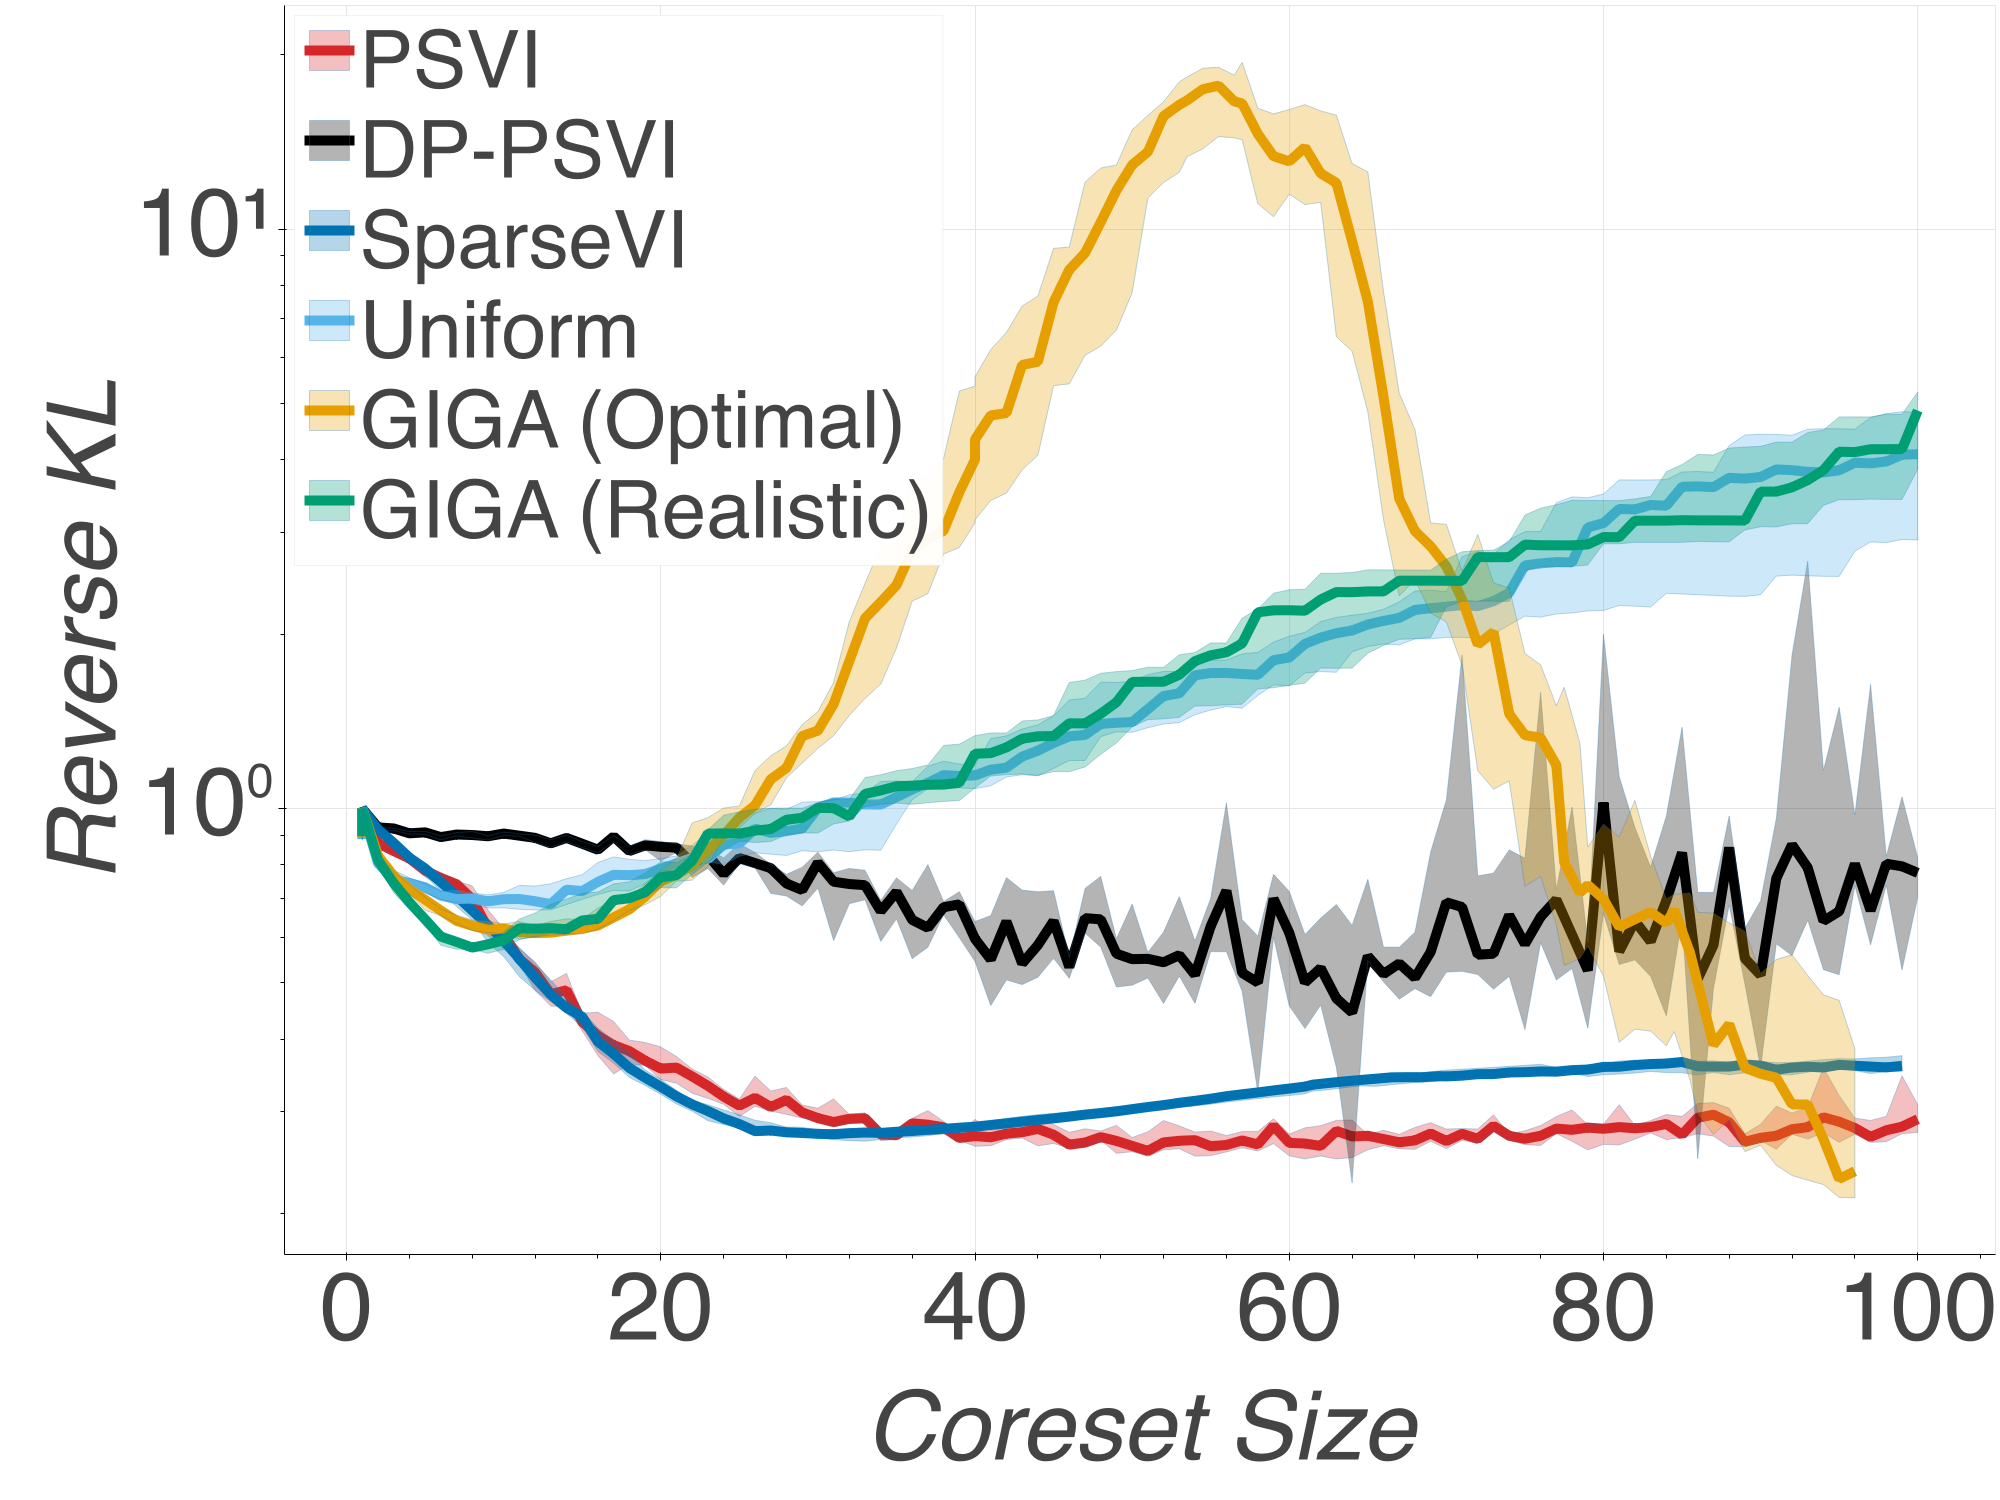
\includegraphics[width=1.15\columnwidth]{\MyPath/figs/wsanta100K_KLDvssz.png}}}%
		\label{sfig:transactions}
	\end{subfigure}\hfill\qquad
	\centering
	\begin{subfigure}[b]{.29\textwidth}
		\subcaption{(b)~\mbox{\textsc{ChemReact100}~($d=100$)}}
		\vspace*{-0.26cm}
		\centerline{\scalebox{1.}{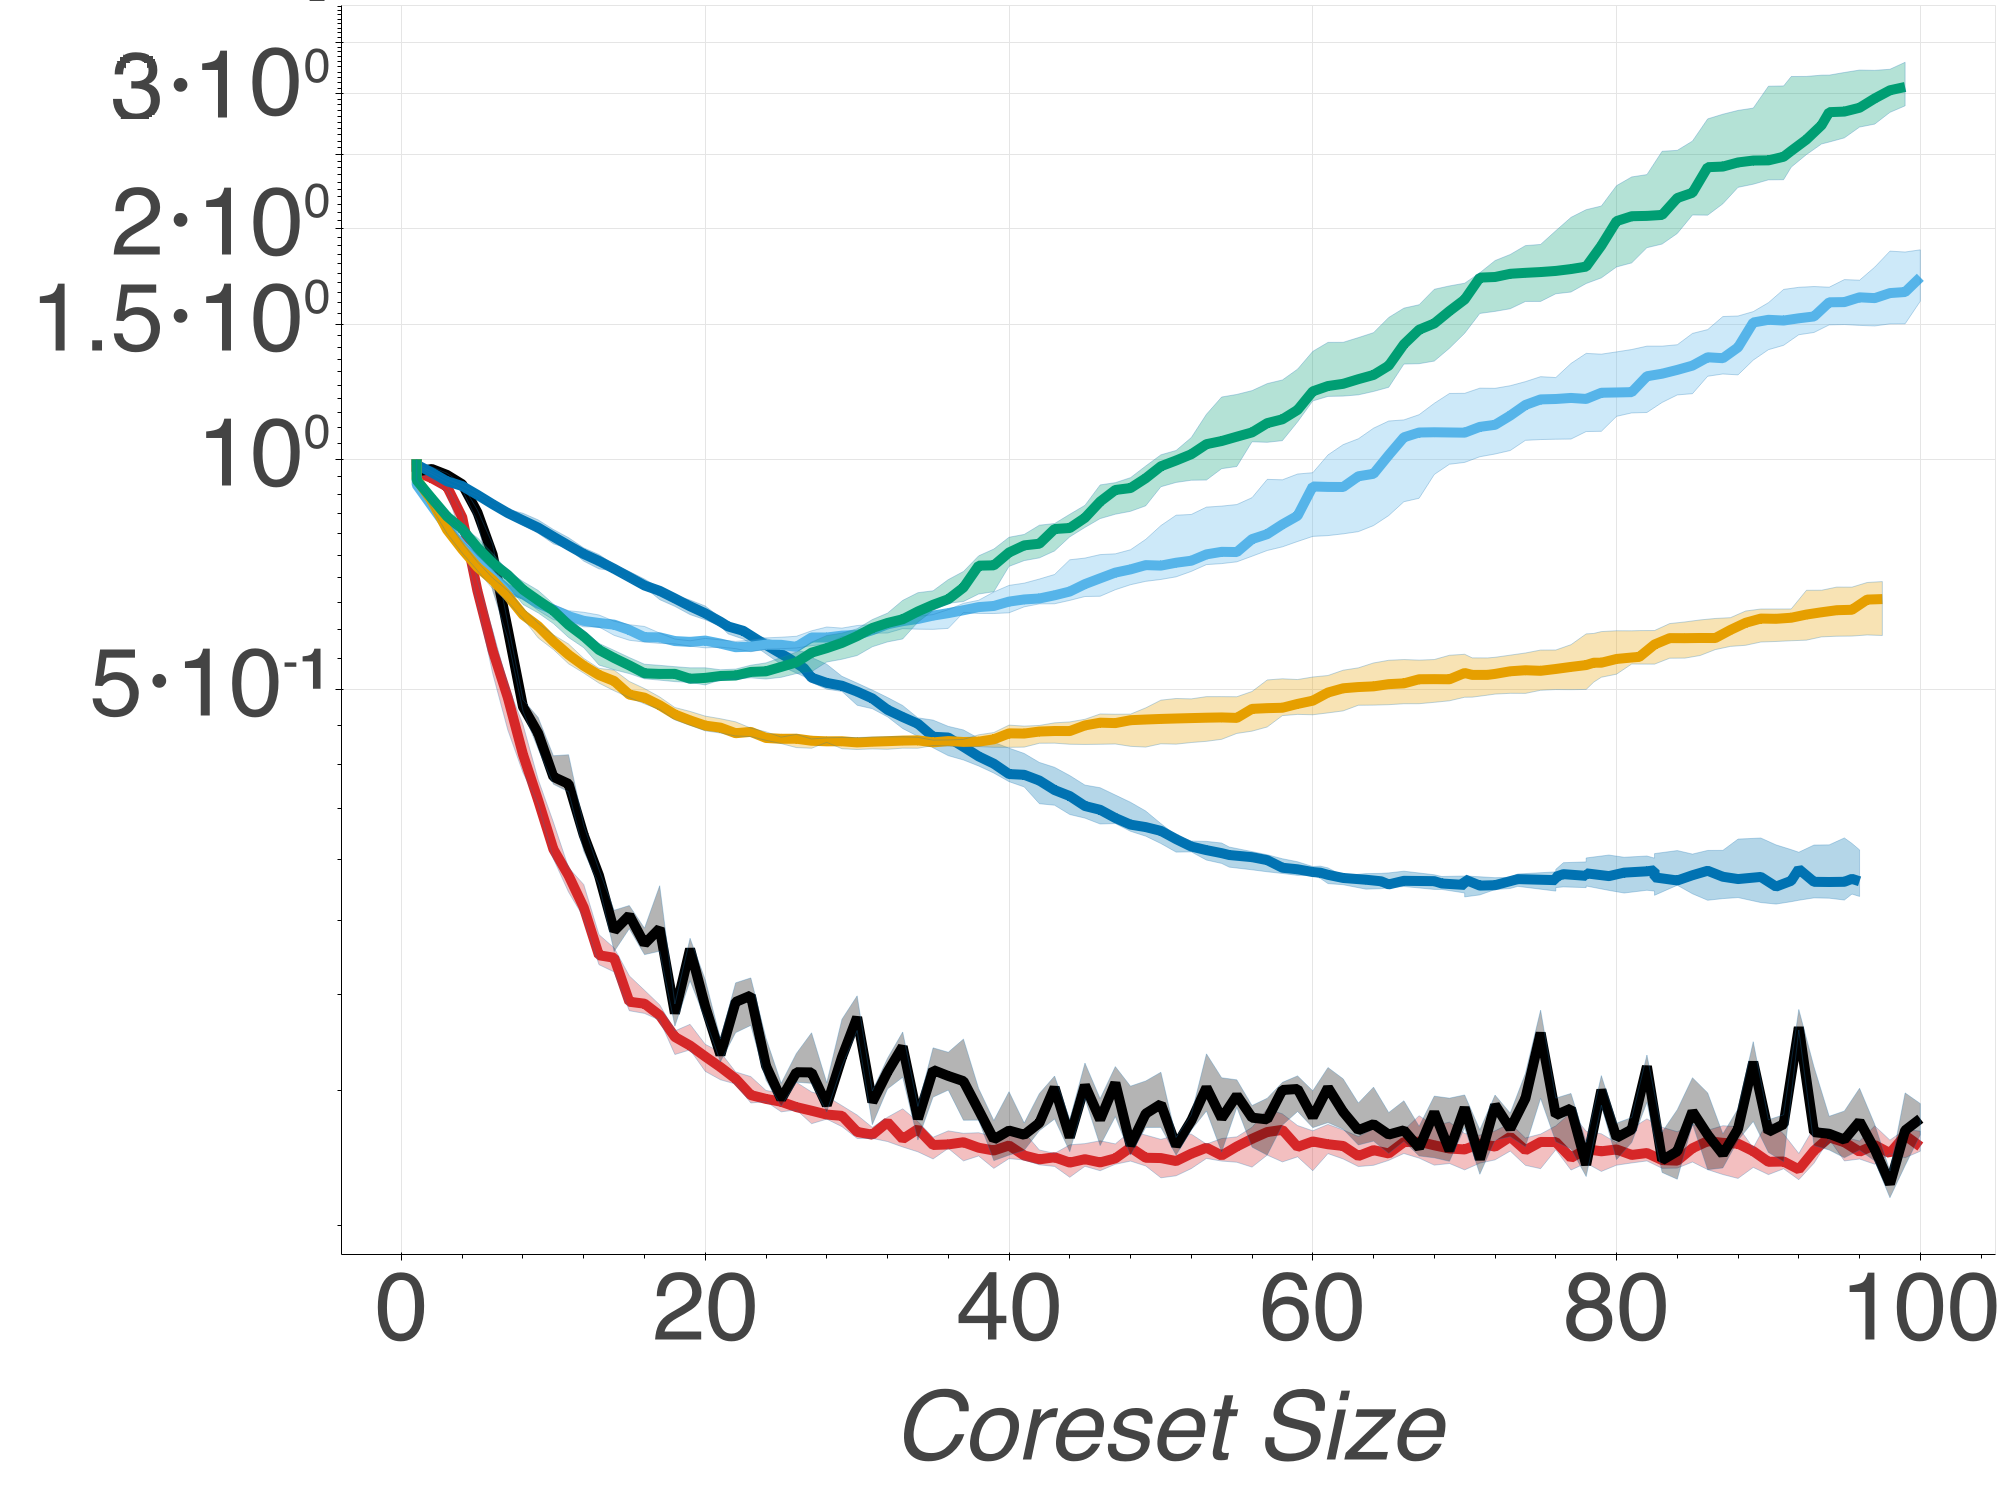
\includegraphics[width=1.15\columnwidth]{\MyPath/figs/wds1100_KLDvssz.png}}}%
		\label{sfig:chemreact100}
	\end{subfigure}\hfill\qquad
	\centering
	\begin{subfigure}[b]{.29\textwidth}
		\subcaption{(c)~\textsc{Music}~($d=237$)}
		\vspace*{-0.26cm}
		\centerline{\scalebox{1.}{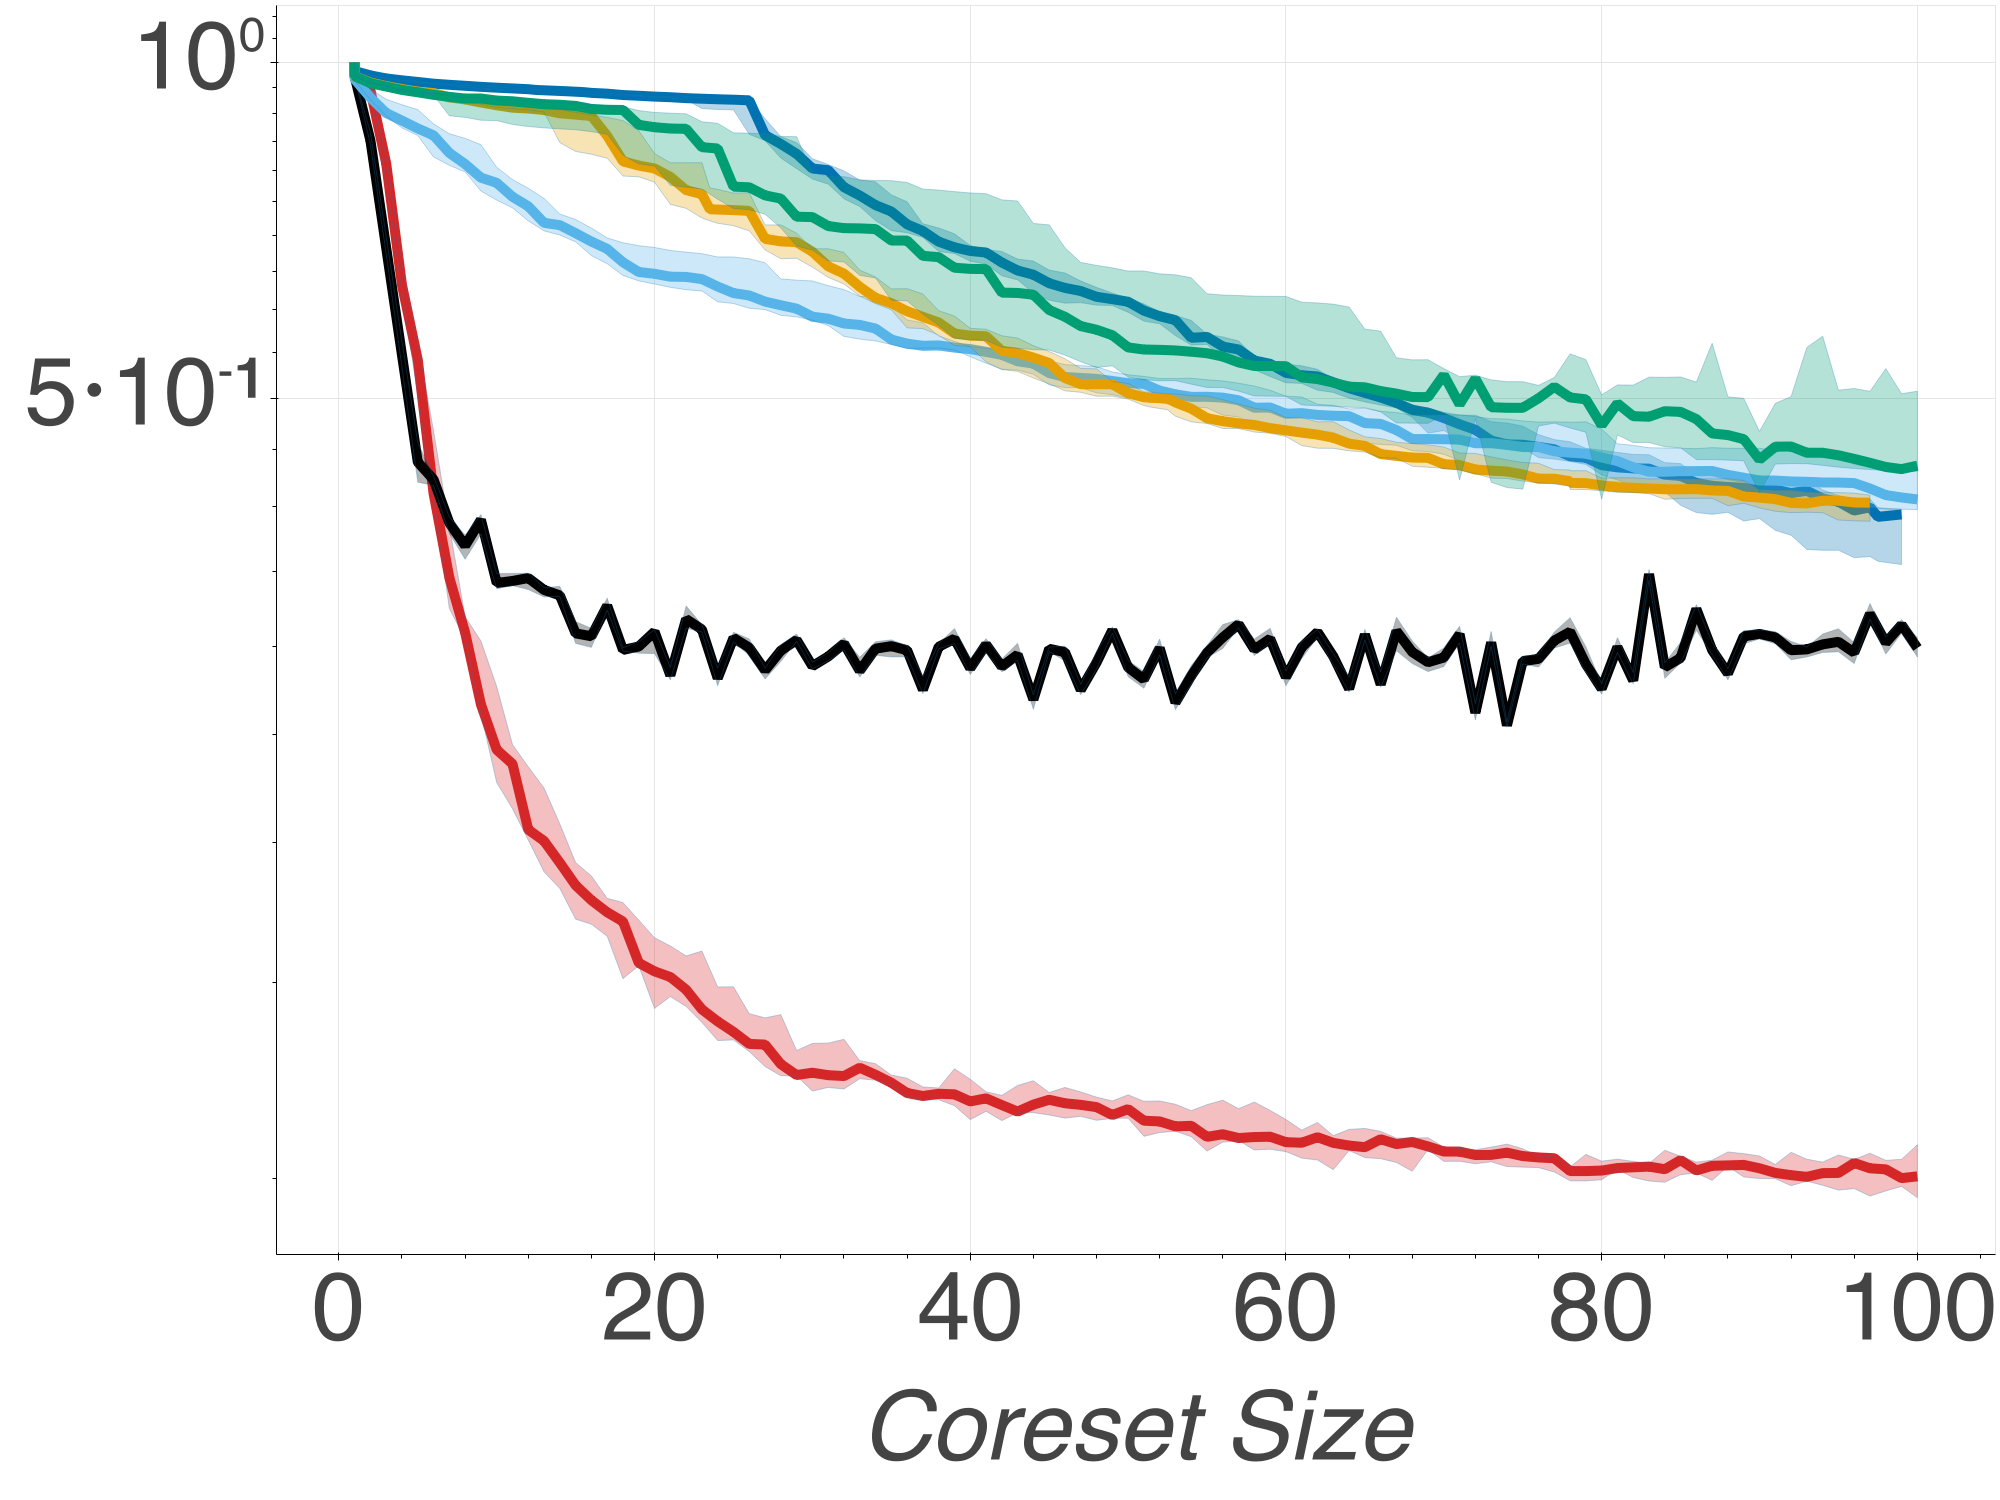
\includegraphics[width=1.15\columnwidth]{\MyPath/figs/wfma_KLDvssz.png}}}%
		\label{sfig:music}
	\end{subfigure}\hfill\qquad
	\caption{Comparison of (pseudo)coreset approximate posterior quality vs  coreset size for logistic regression over 10 trials on 3 large-scale datasets. Presented differentially private pseudocoresets  correspond to $(0.2, 1/N)$-DP. Reverse KL divergence is displayed normalized by the prior.}
	\label{fig:ls_blogreg_dkl}
\end{figure*}


\begin{figure*}[!t]
	\captionsetup[subfigure]{justification=centering}
	\centering
	\begin{subfigure}[b]{.29\textwidth}
		\subcaption{(a)~\textsc{Transactions}}
		\vspace*{-0.26cm}
		\centerline{\scalebox{1.}{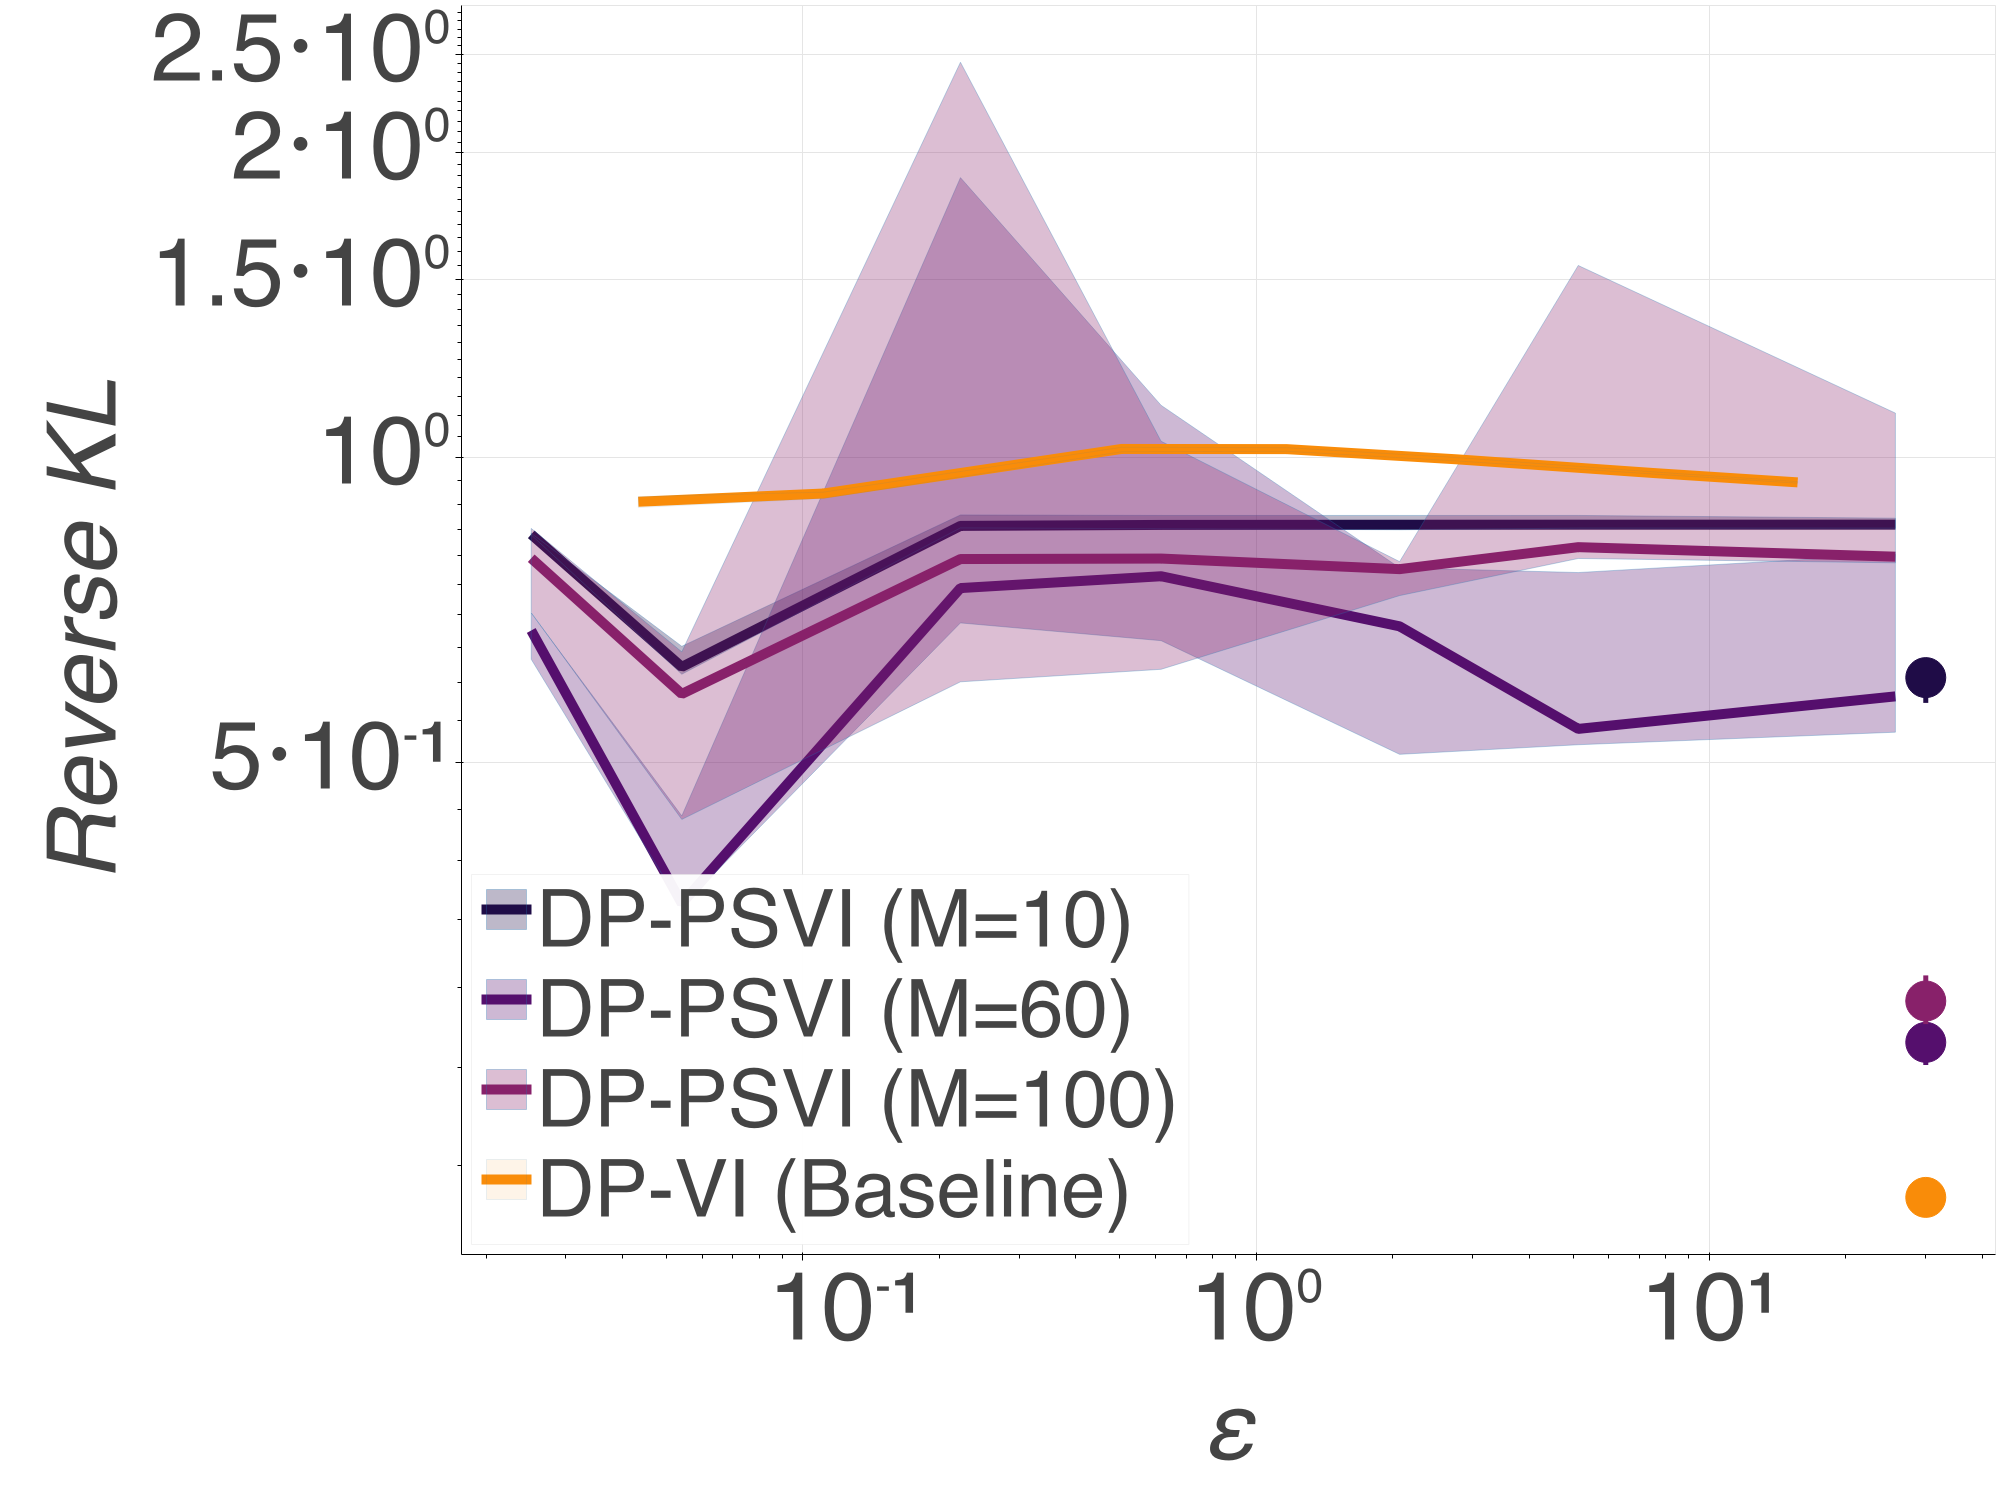
\includegraphics[width=1.15\columnwidth]{\MyPath/figs/wsanta100K_privacy.png}}}%
		\label{sfig:santapriv}
	\end{subfigure}
	\hfill\qquad
	\centering
	\begin{subfigure}[b]{.29\textwidth} 
		\subcaption{(b)~\textsc{ChemReact100}}
		\vspace*{-0.26cm}
		\centerline{\scalebox{1.}{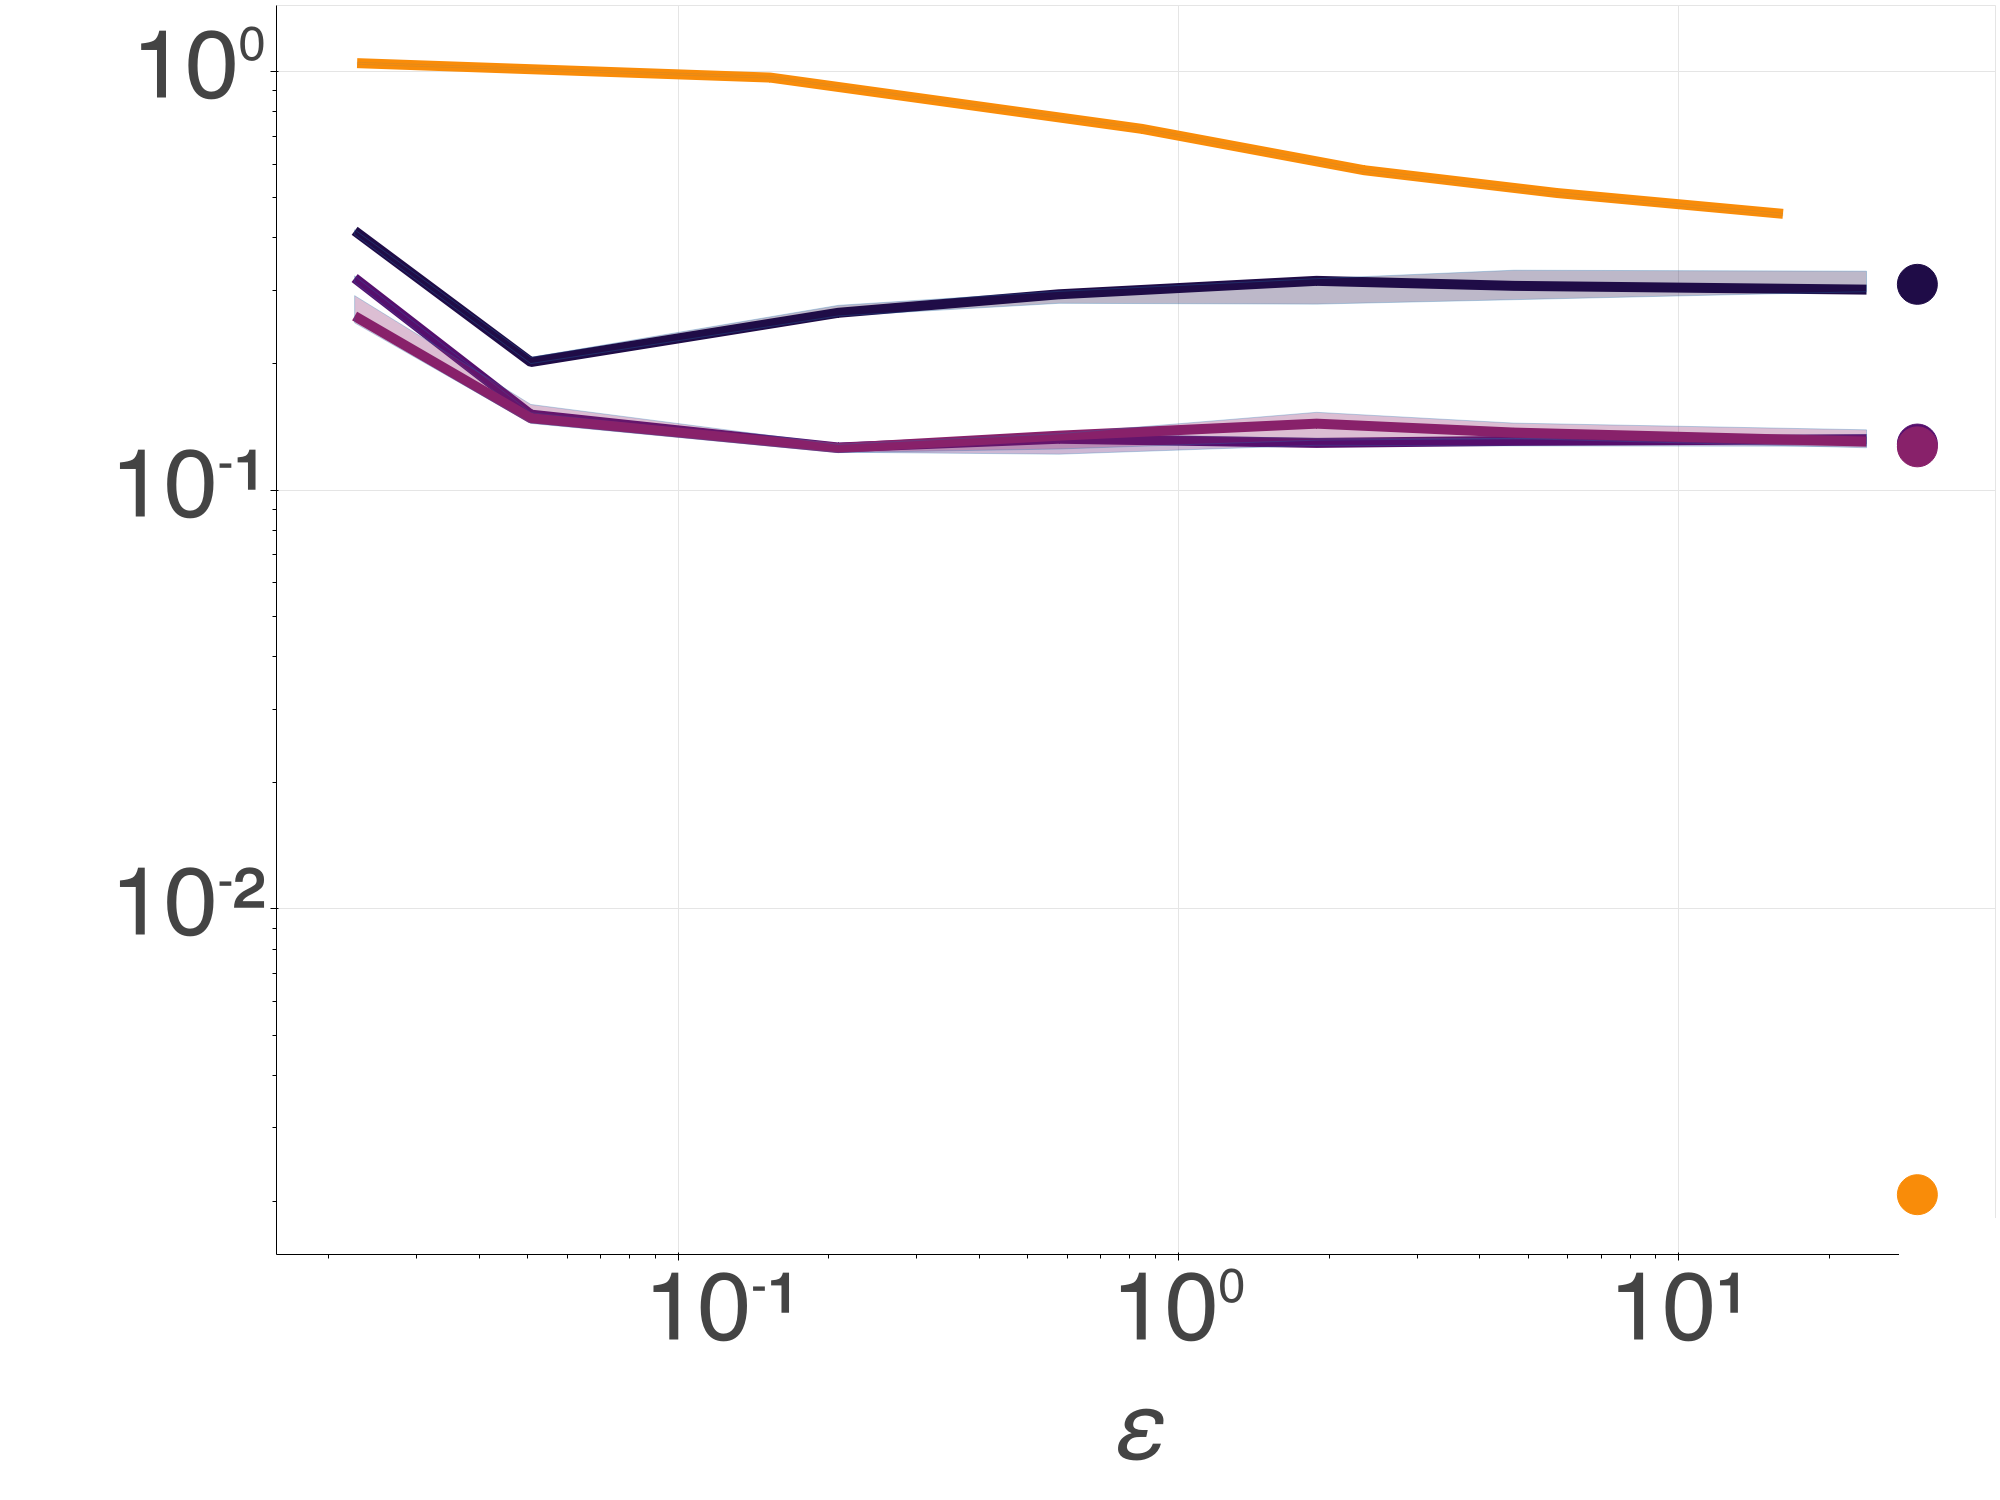
\includegraphics[width=1.15\columnwidth]{\MyPath/figs/wds1100_privacy.png}}}%
		\label{sfig:chemreact100priv}
	\end{subfigure}
	\hfill\qquad
	\centering
	\begin{subfigure}[b]{.29\textwidth}
		\subcaption{(c)~\textsc{Music}}
		\vspace*{-0.26cm}
		\centerline{\scalebox{1.}{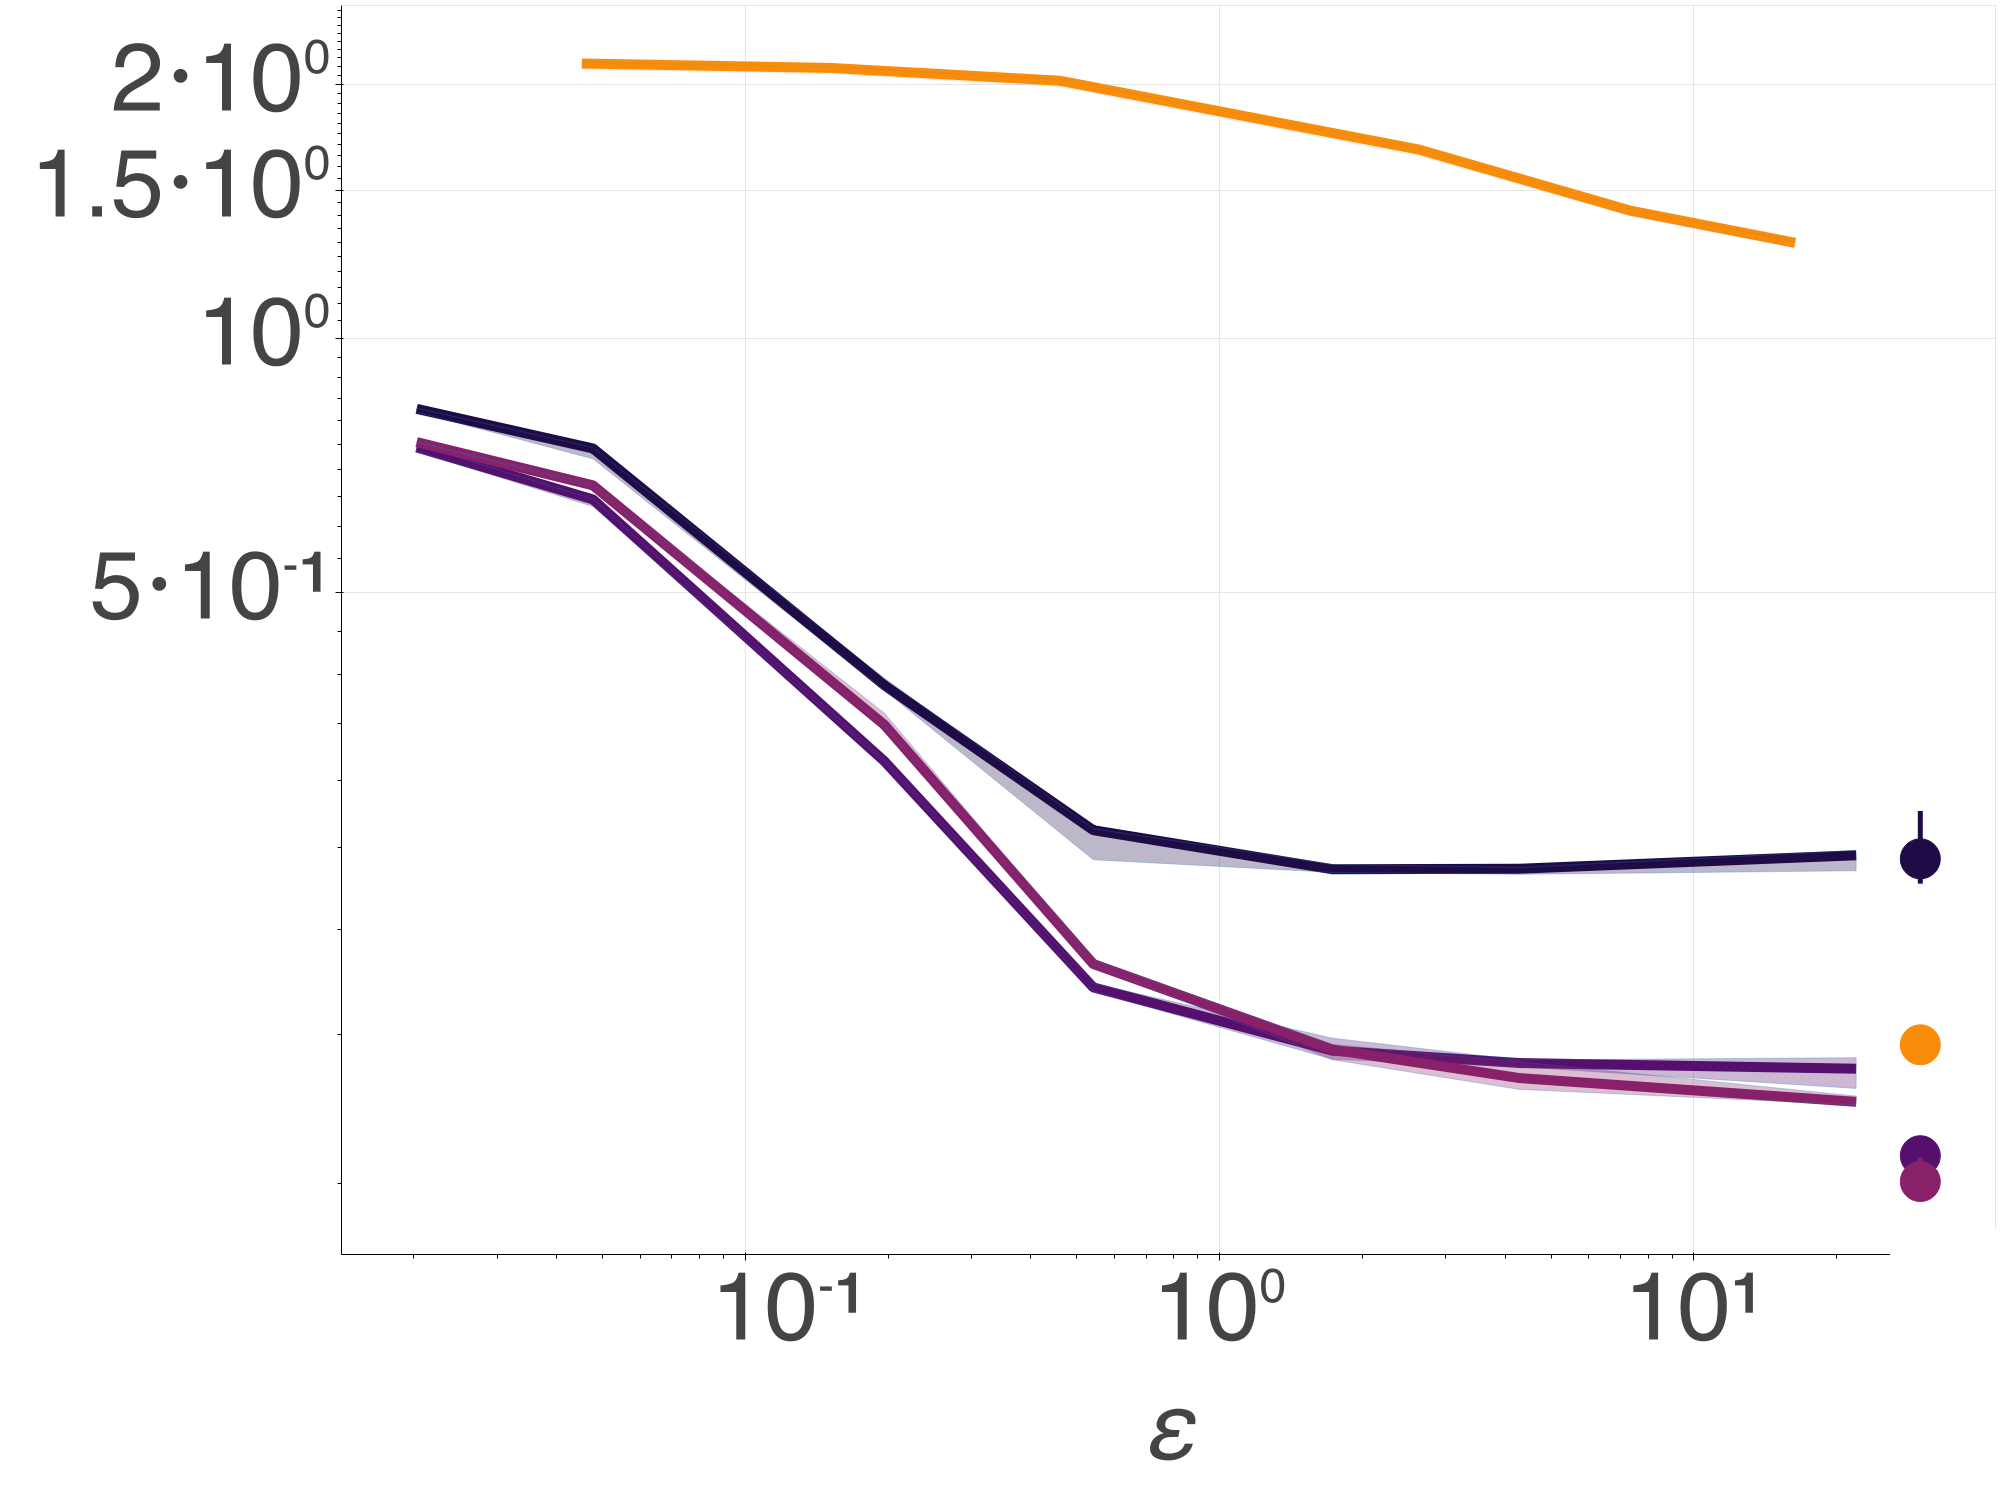
\includegraphics[width=1.15\columnwidth]{\MyPath/figs/wfma_privacy.png}}}%
		\label{sfig:musicpriv}
	\end{subfigure}
	\hfill\qquad
	\caption{Approximate posterior quality over decreasing differential privacy guarantees for private pseudocoresets of varying size plotted against private variational inference~\citep{jalko17}. $\delta$ is always kept fixed at $ 1/N$. Markers on the right end of each plot display the errorbar of approximation achieved by the corresponding nonprivate posteriors. Results are displayed over 5 trials for each construction.}
	\label{fig:dklvseps} 
\end{figure*}


Results presented in~\cref{fig:ls_blogreg_dkl} demonstrate that \psvi~achieves consistently the smallest posterior approximation error in the small coreset size regime, offering improvement
compared to \sparsevi~and being competitive with \gigao,
without the requirement for specifying a weighting function. In~\cref{sfig:transactions}, for $M \geq d$ ~\gigao~follows a much steeper decrease in KL divergence, reflecting the dependence of its approximation quality on dataset dimension per~\cref{prop:original_coreset_fails}. In contrast, \psvi~typically reaches its minimum at $M<d$. The difference in approximation quality becomes clearer in higher dimensions~(e.g. \textsc{Music}, where $d=237$). Perhaps surprisingly, the private pseudocoreset construction has only marginally worse approximation quality compared to nonprivate \psvi~and generally achieves better peformance in comparison to the other state-of-the-art nonprivate coreset constructions. 
In~\cref{fig:dklvseps} we present achieved posterior approximation quality via \dpsvi, against a competitive state-of-the-art method 
%in differentially private variational inference for non-conjugate models 
(\dpvi, \cite{jalko17}). For logistic regression, \dpvi~infers an approximate posterior from the family of Gaussians with diagonal covariance via ADVI~\citep{kucukelbir17}, followed by an additional Laplace approximation. Note that by design, \dpvi~is constrained by the usual Gaussian variational approximation, while \dpsvi~is more flexible and can approach the true posterior as $ M $ increases---this effect is reflected in nonprivate posteriors as well as data dimensionality grows~(see for example~\cref{sfig:musicpriv}). Indeed, we verify that in the high-privacy regime \dpsvi~for sufficient pseudocoreset size (which is typically small for tested real-world datasets) offers posterior approximation with better KL divergence compared to \dpvi. Our findings indicate that private \psvi~offers efficient releases of big data via informative pseudopoints, which enable arbitrary post processing (e.g. running any \emph{nonprivate} black-box algorithm for Bayesian inference), under strong privacy guarantees and without reducing the quality of inference.







